\documentclass[12pt]{report}

\usepackage{amsfonts}
\usepackage{enumitem}
\usepackage{float}
\restylefloat{table}
\restylefloat{figure}

\usepackage[margin=1.5in]{geometry}
\usepackage{graphicx}

\usepackage{setspace}
\doublespacing

\usepackage{titlesec}
\titleformat{\chapter}[display]
    {\normalfont\huge\bfseries}{\chaptertitlename\ \thechapter}{0pt}{\Huge}
\titlespacing*{\chapter}{0pt}{0pt}{10pt}

\bibliographystyle{apalike}

\makeatletter
\renewcommand*\l@chapter[2]{
    \ifnum \c@tocdepth >\m@ne
    \addpenalty{-\@highpenalty}
    \addvspace{1.0em \@plus\p@}
    \setlength\@tempdima{1.5em}
    \begingroup
    \parindent \z@ \rightskip \@pnumwidth
    \parfillskip -\@pnumwidth
    \leavevmode
    \advance\leftskip\@tempdima
    \hskip -\leftskip
    #1\nobreak
    \xleaders\hbox{$\m@th
    \mkern \@dotsep mu\hbox{.}\mkern \@dotsep mu$}
    \hfil\nobreak\hb@xt@\@pnumwidth{\hss #2}\par
    \penalty\@highpenalty
    \endgroup
    \fi
}
\makeatother

\begin{document}

\pagenumbering{roman}

\tableofcontents

%% keep lof and lot on same page
\begingroup
\addcontentsline{toc}{chapter}{List of Figures}
\listoffigures

\let\clearpage\relax
\addcontentsline{toc}{chapter}{List of Tables}
\listoftables
\endgroup

\newpage

\addcontentsline{toc}{chapter}{Summary} %% 1 page

\paragraph This report, titled A Critical Analysis of Learning Styles, provides
a comprehensive overview of some of the most popular models of the theory of
learning styles, as well as a critical analysis as to the suitability of such
methods in a modern educational setting. A general explanation of learning
styles and their proposed benefits will be examined along with an thorough
investigation of the most research papers for each model.

\paragraph Although much effort has been devoted by the scientific community to
ground learning styles in scientific rigor, this report finds that there is an
alarming lack of credible scientific results to correlate the claims put forth
by proponents of learning styles. This report will advise against the direct
application of learning style methods in an educational setting and instead
provide alternative methodology using some of the more tangible results of
learning style theory.

\paragraph While this report attempts to reach definitive, demonstrable
conclusions, it acknowledges the fact that the field of human learning is
highly complex and varied. It is impossible to provide a set of general
recommendations that will benefit everyone.

\chapter*{Introduction} %% 1 page

\addcontentsline{toc}{chapter}{Introduction}
\setcounter{chapter}{1}
\pagenumbering{arabic}

\setlength{\emergencystretch}{3em}

\paragraph Since its recognition in the 1970's, the concept of learning styles
has had a widespread influence on modern education theory, although recently the
credibility of the theory has come under serious question. This report will
first cover the most popular flavours of the learning styles such as Neil
Fleming's VARK \cite{fleming2001teaching}, David Kolb's Experiential Learning
\cite{kolb1984experiential}, and Peter Honey and Alan Mumford's Learning Styles
Questionnaire \cite{honey1989learning}.  The core ideas of learning styles will
be explored, including the proposed benefits such as increased content
retention, and enhanced scores on testable material.

%The author will then
%discuss which learning style is most descriptive of their own personal learning
%habits.

\setlength{\emergencystretch}{0em}

\paragraph After discussing the most prevalent models of learning styles, this
report will then present the modern critique of the theory. Although learning
styles have existed for a substantial period of time, there is an alarming lack
of scientifically rigorous study confirming the claims touted by proponents of
the theory. Though there have been attempts to ground the theory in factual,
reproducible experimentation, none have provided a satisfyingly conclusive
answer to the question of whether the application of learning style based
theory in an educational setting provides measurable benefit to the learning
process.  This report will draw its own conclusions as to the suitability of
learning styles as an educational tool, and provide recommendations for any
readers interested in employing a model of learning styles in an educational
setting.

%% BODY 4-6 pages

\chapter*{An Overview of Learning Styles}
\addcontentsline{toc}{chapter}{An Overview of Learning Styles}
\setcounter{chapter}{2}

\paragraph Although many distinct models of learning styles exist, they share a
core theme. Learning styles are broadly described as ``cognitive, affective,
and physiological traits that are relatively stable indicators of how learners
perceive, interact with, and respond to the learning environment''
\cite{keefe1990developing}. This suggests that an individual will be able to
learn at an increased rate, or with higher content retention, if they are
taught in a way that aligns with an innate personal preference for consuming
information.

\section {VARK Model}

\paragraph One well known model is Neil Fleming's \textit{Visual, Auditory,
Reading/Writing, Kinesthetic} or VARK model \cite{fleming2001teaching}.
Fleming himself describes VARK as ``a starting place for a conversation among
teachers and learners about learning" \cite{fleming2006learning}. VARK attempts
to classify an individual learner into the sensory category from which they
benefit the most. Although it is possible for a learner to be competent using
more than one sensory aspect, Fleming claims that information can be consumed
most efficiently when the dominant learning style of a student is thoroughly
utilized.

\begin{figure}[H]
    \centering
    \includegraphics[width=5in]{figures_tables/vark}
    \caption{The VARK model}
\end{figure}

\paragraph The model claims visual learners can learn best when consuming
content visually, through pictures, visual aids such as overhead slides,
blackboard visuals graphs, or diagrams. Auditory learners benefit from
listening to lectures, oral discussions, or tapes. Learners of the
reading/writing variety benefit most from committing their ideas to paper, note
taking, and relevant reading material.  Finally, kinesthetic learners prefer to
learn via physical activities, such as touching and experimenting.

\section{Experiential Learning Model}

\paragraph One of the oldest models of learning styles, proposed in 1984, is
American educational theorist David Kolb's Experiential Learning Model
\cite{kolb1984experiential}. This model outlines two related approaches for
\textit{grasping} experience: Concrete Observation and Abstract
Conceptualization, as well as two other related approaches for
\textit{transforming} experience: Reflective Observation and Active
Experimentation. The theory describes a cyclical model of learning that
provides a feedback loop where "knowledge is created through the transformation
of experience" \cite{kolb1984experiential}.

\begin{figure}[H]
    \centering
    \includegraphics[width=5in]{figures_tables/kolb}
    \caption{The Experiential Learning model}
\end{figure}

\paragraph Using these four types of experiential learning, Kolb devised a
learning style inventory which can be used to identify four unique methods of
learning based on which experiential approach is dominant. Each style of
learning represents a choice. As it is impossible to simultaneously play an
instrument (Concrete Experience) and read an instructional book on guitar
playing (Abstract Conceptualization), it is necessary to resolve the conflict
by making a choice between the two methods. As one begins developing a
preference as to which method of learning one is best suited, this accumulated
characteristic becomes what is known as an Experiential Learning style.

\begin{singlespacing}
    \begin{table}[H]
        \hspace{-0.5in}
        \begin{tabular}{|c|p{2in}|p{2.5in}|}
            \hline
            \textbf{Learning Style} & \textbf{Learning Characteristic} & \textbf{Description} \\ \hline
            \textbf{Converger} & Abstract Conceptualization \newline + Active Experimentation &
            - strong in practical application of ideas \newline
            - can focus on deductive reasoning on specific problems \newline
            - unemotional \\ \hline
            \textbf{Diverger} & Concrete Experience \newline + Reflective Observation &
            - strong imaginative ability \newline
            - interested in people \newline
            - good at generating ideas and seeing things from different perspectives \\ \hline
            \textbf{Assimilator} & Abstract Conceptualization \newline + Reflective Observation &
            - strong ability to create theoretical models \newline
            - concerned with abstract concepts rather than people \newline
            - excels in inductive reasoning \\ \hline
            \textbf{Accommodator} & Concrete Experience \newline + Active Experimentation &
            - greatest strength is doing things \newline
            - solves problems intuitively \newline
            - performs well when required to react quickly \\ \hline
        \end{tabular}
        \caption{Kolb's learning style inventory}
    \end{table}
\end{singlespacing}

\pagebreak

\section{Honey and Mumford Model}

\paragraph The Honey and Mumford model of learning styles is derived directly
from Kolb's Experiential Learning model, with some changes made to address
insufficiencies when dealing with the managerial experiences of decision making
and problem solving.

\begin{figure}[H]
    \centering
    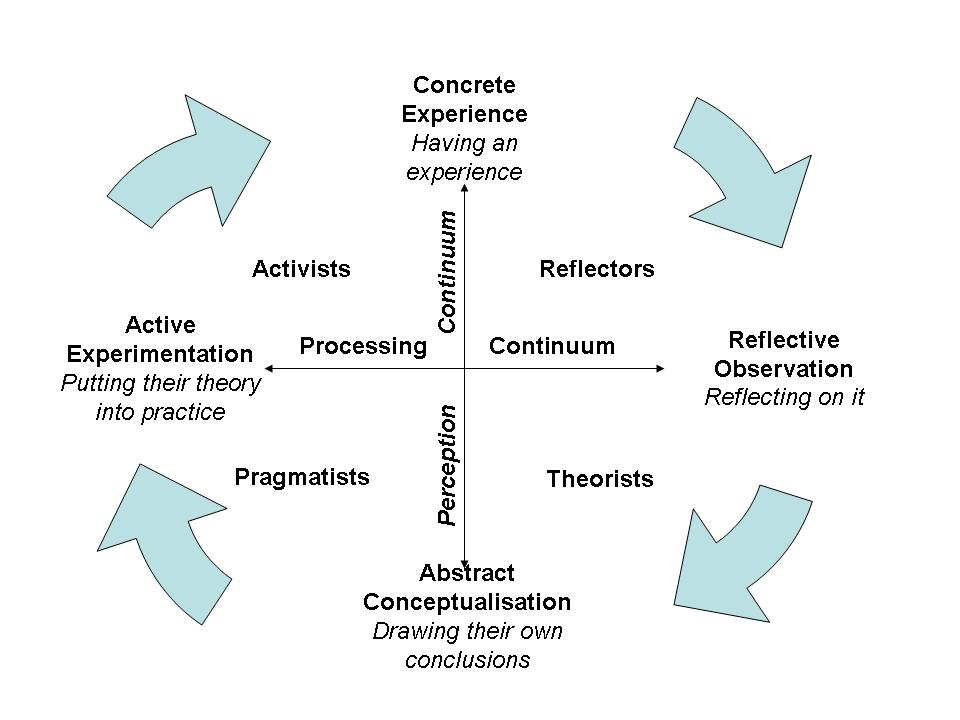
\includegraphics[width=5in]{figures_tables/honey_mumford}
    \caption{The Honey and Mumford model}
\end{figure}

\paragraph Honey and Mumford used the learning style inventory of the
Experiential Learning model and produced the Learning Styles Questionnaire: a
simple agree/disagree questionnaire designed to help uncover learning
preferences in individuals who have may not have ever given any consideration
as to how they learn best.

\chapter*{Analysis of My Learning Style}
\addcontentsline{toc}{chapter}{Analysis of My Learning Style}
\setcounter{chapter}{3}

\paragraph Using the Kolb Experiential Learning Model, the author of this report
would fall into Abstract Conceptualisation category. As a mathematics student,
much of my work directly involves abstract conceptualisation to comprehend
highly abstract mathematical concepts. Very little in mathematics could be
considered to fall under the Active Experimentation, Concrete Experience, or
Reflective Observation categories. As such, I have developed a preference for
this abstract model of learning, and prefer to learn new topics using a
high-level, conceptual approach. Once I have a solid grasp on the high-level
aspects of a new concept, I find it much easier to concretely apply those
concepts in practice.

\paragraph The Kolb Learning Style Inventory learning style categorizes me as an
Assimilator: strong ability for theoretical modeling, concerned with abstract
concepts, and excellent inductive reasoning. All of these are useful traits for
a student in mathematics. The Assimilator style emphasizes Abstract
Conceptualisation and Reflective Observation, which I think is a reasonable
description of myself, as I often reflect on experiences after the fact, in
order to gain a better understanding.

\chapter*{Critique of Learning Styles}
\addcontentsline{toc}{chapter}{Critique of Learning Styles}
\setcounter{chapter}{4}

\paragraph Although the theory of learning styles claims to be able to provide
a more effective and efficient educational model, there is a significant lack
of rigorous scientific research to support these claims. In order to properly
demonstrate the benefits of a learning style model, it is necessary to first
identify the individual learning style of a student according to the model
which is under scrutiny and then randomly assign the student to any of the
learning methods included in the model. The student's performance on a variety
of tasks would then be thoroughly tested before and after instruction in order
to determine what effect the application of a particular learning style had on
the student.

\paragraph However, researchers find that studies designed to test the benefits
of learning styles have failed to use the type of randomized research
strategies that would ensure scientifically credible results. An article
published for the Association of Psychological Science states:

\begin{quote}
    We found virtually no evidence for learning styles$\dots$ very few studies
    have even used an experimental methodology capable of testing the validity
    of learning styles applied to education. Moreover, of those that did use an
    appropriate method, several found results that flatly contradict the popular
    hypothesis" \cite{pashler2008learning}.
\end{quote}

\noindent Even though the authors of the article did find one experimental
study which was conducted in such a way as to potentially provide strong
evidence for the learning style hypothesis, that study was not without flaws.
The study tested 324 ``gifted and talented" high-school students using the
Sternberg Triarchic Abilities Test \cite{sternberg1993sternberg}, which rates
each student's analytical, creative and practical abilities. Based on the test
results, a subset of students were assigned to groups where they received
instruction tailored to their specific area of strength. The study found that
``after the data were screened for deviant scores, matched subjects reliably
outscored mismatched subjects on two of the three kinds of assessments."
\cite{sternberg1996identification}.

\paragraph Unfortunately, the study suffers from some serious methodological
issues. The positive correlation between the method of instruction and higher
test results was only achieved after some significant post-processing: removing
the deviant scores mentioned above. As well, the final test scores used to
determine a subject's improvement were never reported.

\paragraph In other cases, research efforts could find no positive relationship
between the application of a learning style method and actual enhanced
learning.  Studies such as Massa and Mayer \cite{massa2006testing} and
Constantinidou and Baker \cite{constantinidou2002stimulus}, find no reason to
believe the practical application of learning styles has a positive impact on
learning.

\chapter*{Conclusions and Recommendations}
\addcontentsline{toc}{chapter}{Conclusions and Recommendations}
\setcounter{chapter}{5}
\setcounter{section}{0}

\section{Conclusions} %% at least 3 conclusions

\paragraph Learning styles have been a popular idea throughout modern education
theory and, while much effort has been put into producing a large body of
research regarding the theory, there has yet to be any scientifically credible
experimentation to affirm the claims. Too few of the studies conducted are
rigorous or methodological enough to hold up to scientific scrutiny. The few
that can often produce results that do not support the learning styles
hypothesis. As such, there is currently little scientific credibility lent to
the idea that the use of learning styles in a modern education setting provides
any kind of beneficial effect.

\paragraph While these deep rooted issues with learning styles are certainly
troubling, there are also flaws that can arise during the implementation of a
learning style method. Most commonly, learning style questionnaires are used to
measure an individual's learning style preference. However this is inherently
biased. Self-reports such as these very rarely produce a true sampling of
learning behaviour, but instead reflect the learner's own impression of how they
learn, or an similarly influenced impression which may be affected by what the
subject thinks the conductor of the questionnaire wants to hear. Methods such as
these learning style questionnaires or other such self evaluations cannot be
used as a reliable instrument with which to conduct research and thus the
results of studies conducted using these sub-par methods can not be considered
reliable.

\section{Recommendations} %% at least 2 recommendations

\paragraph The author advises any readers interested in education theory and
the psychology behind human learning to think critically about the theory of
learning styles. Before blindly incorporating learning style based methods into
a curriculum or educational program, consider first the lack of credible
results regarding the proposed benefits of the theory. Many studies conclude
that the positive effect of a learning style based curriculum is negligible,
and thus the resources spent investing in the program are wasted.

\paragraph While the application of learning styles cannot be shown to produce a
tangible improvement in the learning process, what can be taken from the theory
is that the process of human learning exists as an incredibly varied spectrum of
possibilities. Instead of narrowing one's focus on one perceived "special"
section of this spectrum, it is wise to instead attempt to incorporate a
multitude of methods in order to provide a rich, varied curriculum that will
engage a wide audience of learners. The author recommends that one take into
account the important characteristics of learning that each learning style
method has classified and tailor an educational program to target these
characteristics in concert rather than isolation. Instead of hoping to find
gains on an individual level, this approach will allow you to create a learning
process that provides benefit to a deeper range of learners.

\bibliography{references}

\chapter*{Appendices}

Your report must:

\begin{itemize}[label={\checkmark}]
    \item{Include 4-6 pages of body content. Figures or tables that are included
        in the body are excluded in the 4-6 page count. Adherence to the 3Cs (clarity, conciseness, and coherence)
        will allow you to meet this page limit}
    \item{Include at least one table}
    \item{Include at least one figure}
    \item{Use a 12-point serif font}
    \item{Be double-spaced}
    \item{Be written in formal, standard English, with no contractions}
    \item{Be spell-checked and proofread}
    \item{Include pages numbered according to the conventions described in the Report Resources tab}
\end{itemize}

\noindent Your report must conform to the format and conventions described in the Report
Resources page.  You do not have to bind your report or include a front cover
because you will submit your report to us online.  Your report will include the
following pages and sections:

\begin{itemize}[label={\checkmark}]
    \item{Title page}
    \item{Letter of submittal (addressed to the PD2 course instructor)}
    \item{Table of contents}
    \item{List of Figures and Tables, if appropriate}
    \item{Summary}
    \item{Introduction}
    \item{Body (that includes both an objective analytical component and a reflective component)}
    \item{Conclusions (the section is ``conclusions" as in ``findings", not ``conclusion")}
    \item{Recommendations (specific, measurable, and attainable)}
    \item{Reference}
    \item{Appendices (you need at least one appendix which includes this checklist)}
\end{itemize}

\end{document}
